\section{Overview}\label{sec:overview}

\begin{figure}
  \centering
  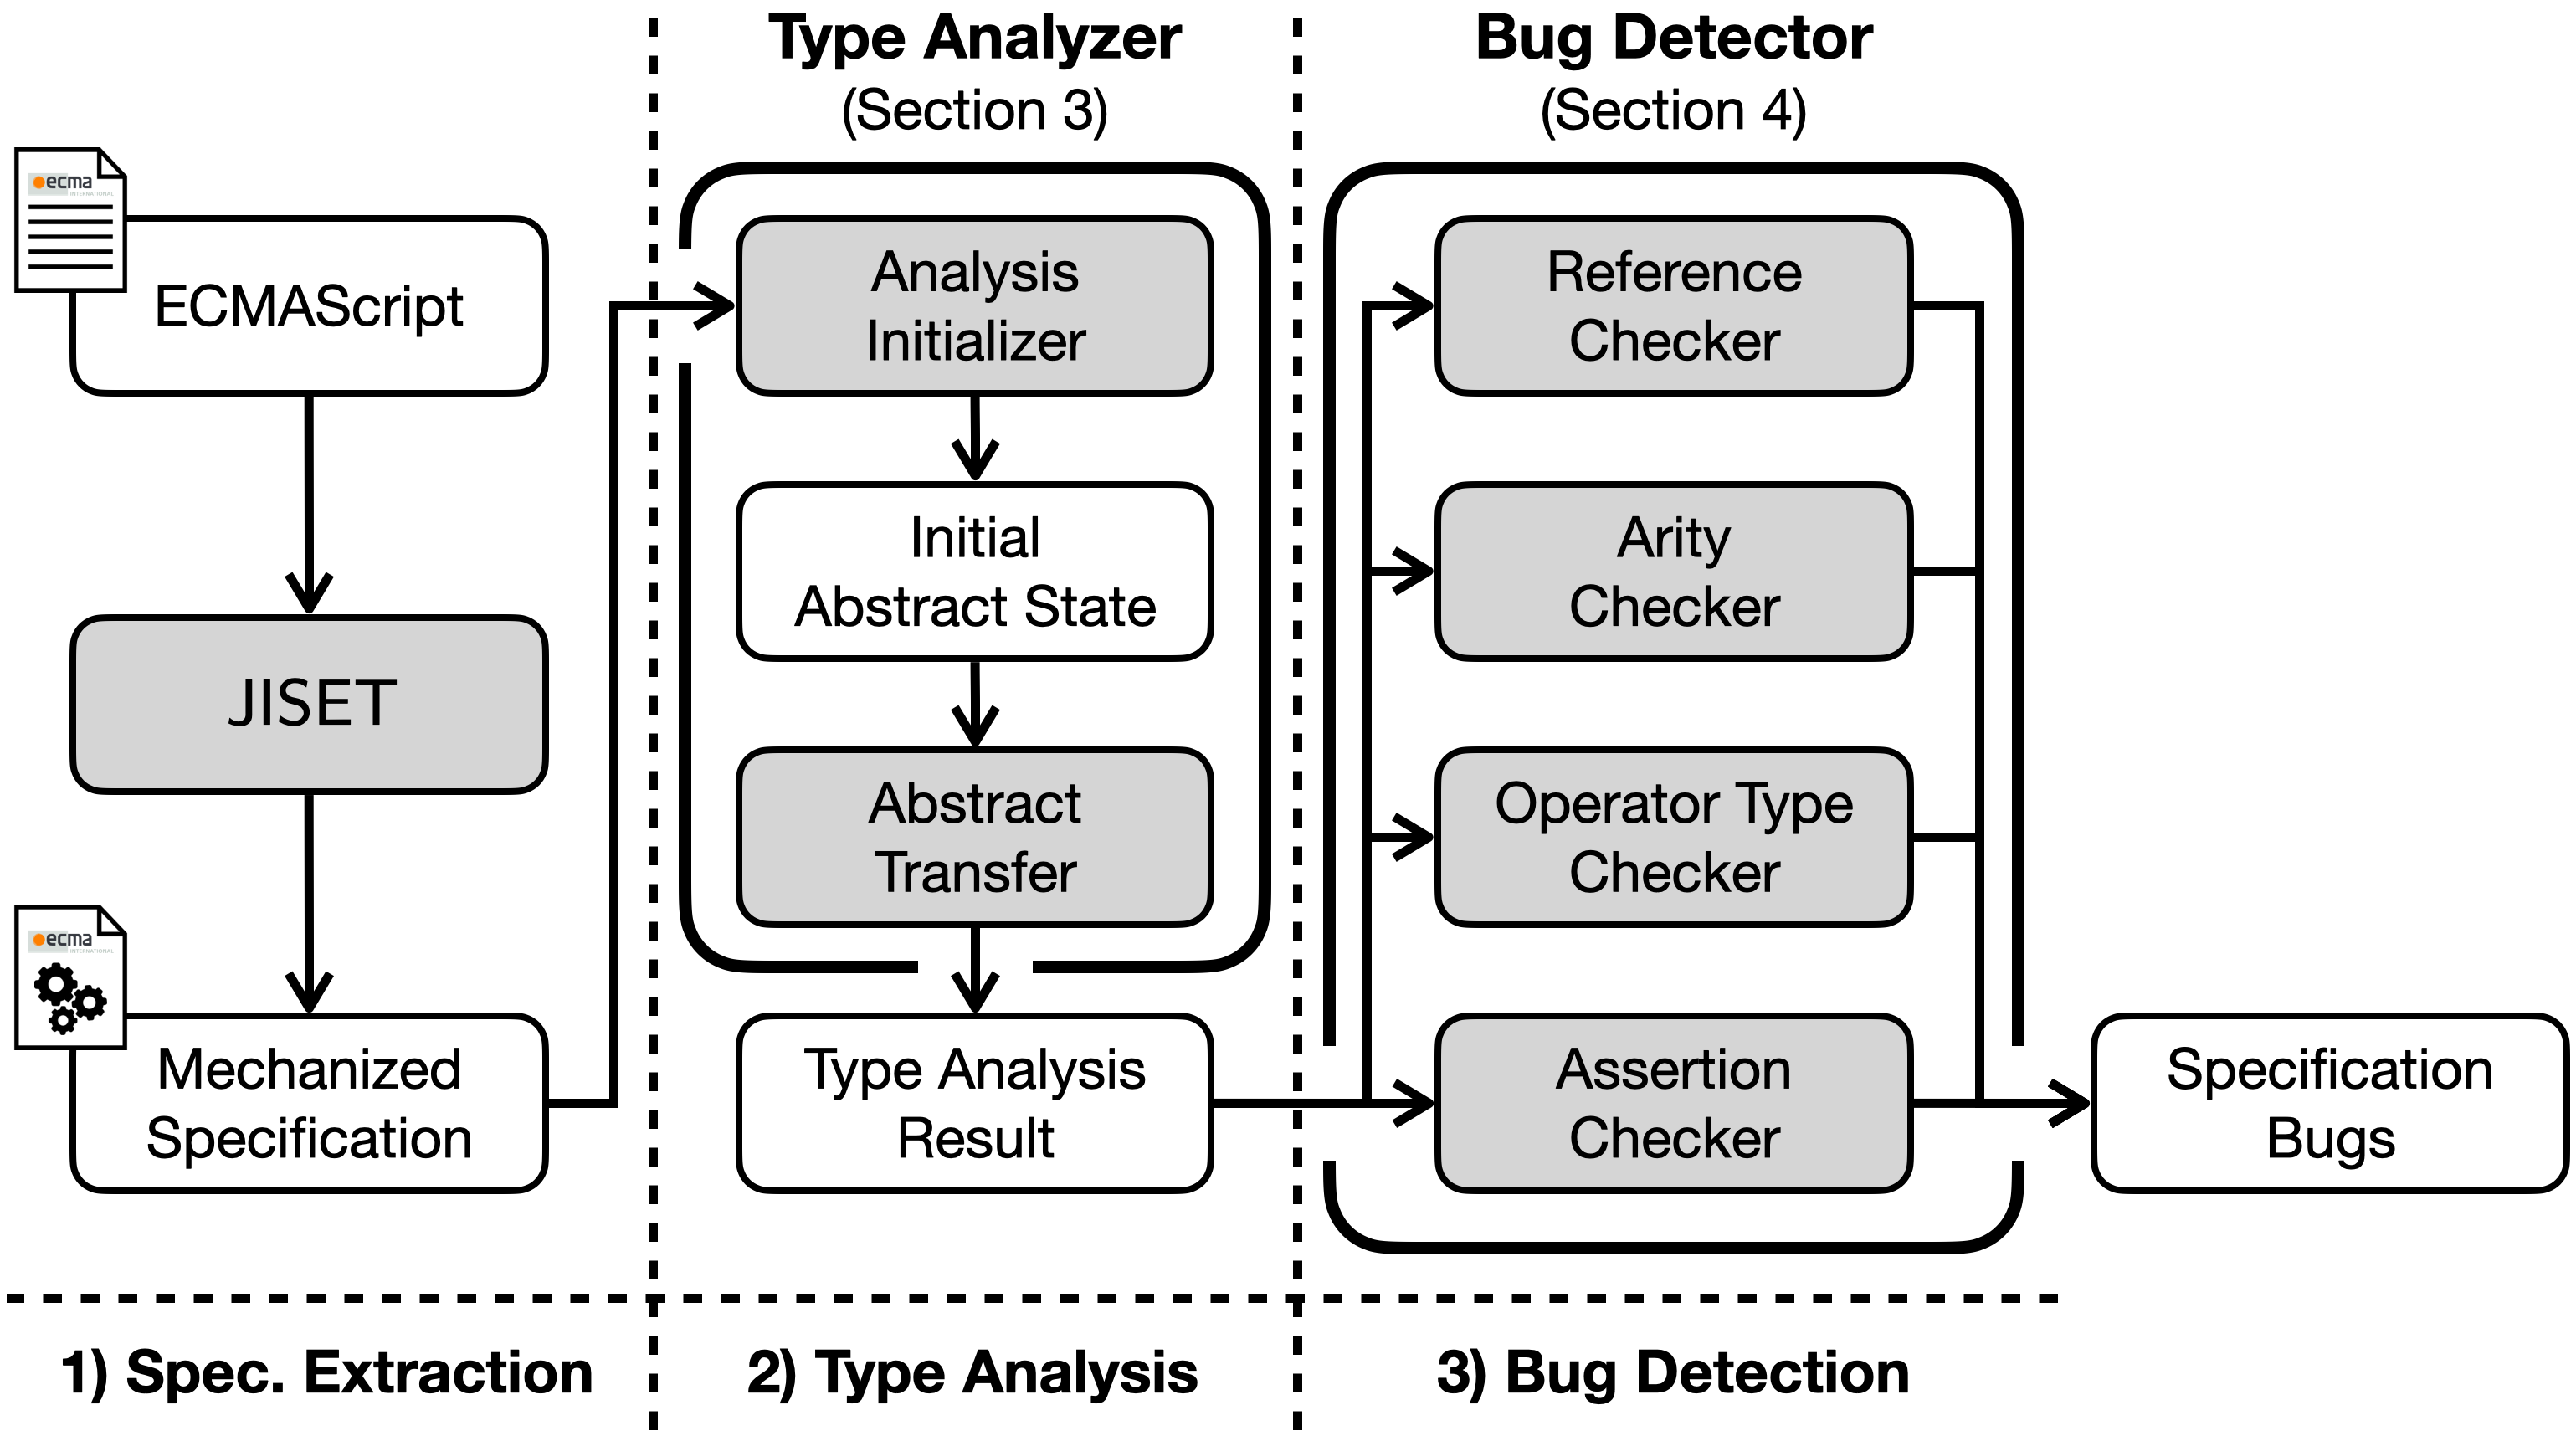
\includegraphics[width=\columnwidth]{img/overall}
  \caption{$\tool$: a type analyzer and a bug detector for
  mechanized specifications extracted from ECMAScript by $\jiset$}
  \label{fig:overall}
  \vspace*{-1.5em}
\end{figure}

\begin{figure*}[t]
  \centering
  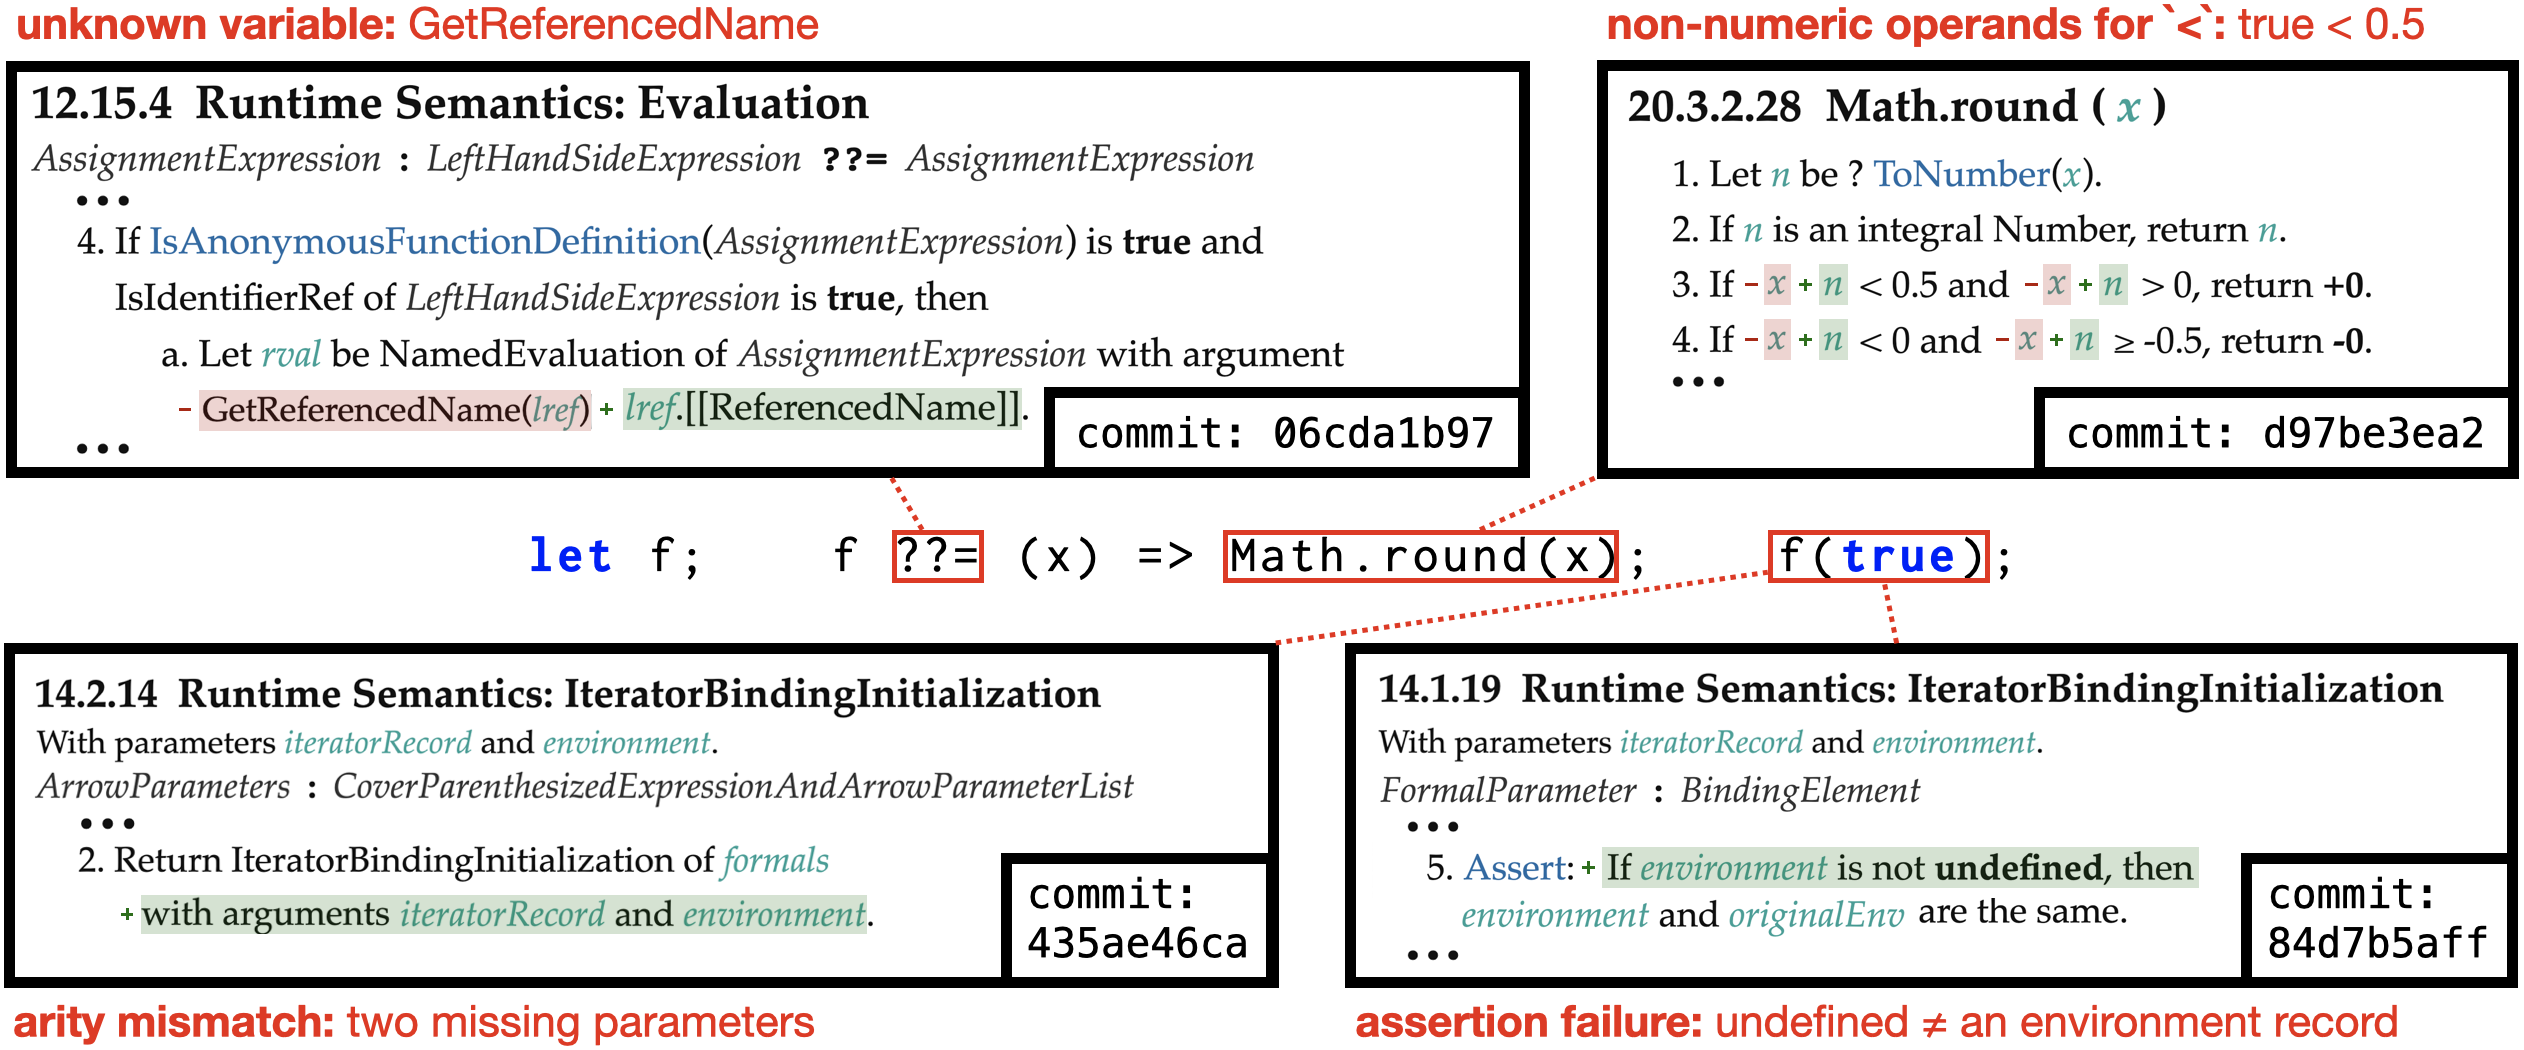
\includegraphics[width=.9\textwidth]{img/example}
%  \vspace*{-1.5em}
  \caption{An example JavaScript program with related previous specification
  bugs and their bug fixes}
  \label{fig:example}
  \vspace*{-1.5em}
\end{figure*}
% XXX
% \begin{lstlisting}[style=FigureJS]
% let f;    f ??= (x) => Math.round(x);    f(true);
% \end{lstlisting}

In this section, we demonstrate the overall structure of $\tool$ depicted in
Figure~\ref{fig:overall}.  It consists of three components:
1) specification extraction, 2) type analysis, and 3) bug detection.


\subsection{Specification Extraction}\label{sec:overview-spec-extract}
$\tool$ extracts the JavaScript syntax and semantics using $\jiset$,
and it extracts specification types from ECMAScript.

\paragraph{Syntax and Semantics}
ECMAScript uses a variant of extended BNF notations to describe the JavaScript syntax.
While $\jiset$ synthesizes AST structures and JavaScript parsers from
the lexical and syntactic productions in ECMAScript, $\tool$ uses only
AST structures to define their types and access corresponding syntax-directed algorithms.
ECMAScript uses abstract algorithms written in a structured natural language to
describe the JavaScript semantics.  $\jiset$ compiles such abstract algorithms to
$\ires$ functions with parameters and local variables.  For example, the
algorithm step
``\raisebox{-0.55ex}{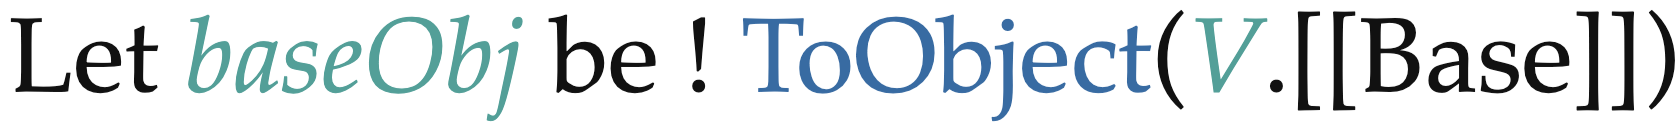
\includegraphics[width=0.55\columnwidth]{img/compile-example}}''
is compiled to an $\ires$ instruction $\kwlet \; \code{baseObj} \code{=}
\escaped\!  \code{ToObject(V.Base)}$.  To make it more suitable for type
analysis, we modify $\ires$ as formally defined in Section~\ref{sec:ires}.

\paragraph{Types}
In addition to JavaScript types,
$\tool$ represents three kinds of specification types.
First, because ASTs are values in abstract algorithms, 
they can be stored in variables and passed as function arguments.
For ASTs, we use their production names as their
types and automatically link their corresponding syntax-directed algorithms as their fields.
Second, ECMAScript supports various record types and fields
whose possible values are defined in their corresponding tables.
For example, ``Table 9: Completion Record Fields'' in the latest
ECMAScript describes the fields of the completion records.
% The newest version contains tens of tables for record types, and they are backward compatible in general.
Thus, we manually model the fields of record types based on the tables
in the latest version and use them in a type analysis.
Third, for list-like structures, we define the empty list type
$\clist{}$ and parametric list types $\clist{\tau}$.

\subsection{Type Analysis}\label{sec:overview-type-analysis}

$\tool$ performs a type analysis with flow-sensitivity and
type-sensitivity for arguments.
Each function is split into multiple flow- and type-sensitive views, and an
abstract state stores mapping from views to corresponding abstract environments.
To handle views separately, we use a worklist algorithm.
The type analyzer consists of two sub-modules: an \textit{analysis initializer} and an
\textit{abstract transfer function}.

\paragraph{Analysis Initializer} It defines the initial abstract state and the
initial set of views for a worklist. ECMAScript provides three
kinds of abstract algorithms: \textit{normal}, \textit{syntax-directed}, and
\textit{built-in}. Since syntax-directed algorithms and built-in algorithms have
their parameter types, we use them as entry points of type analysis.  For each entry point, the
initializer defines its abstract environment with parameter types and adds the
flow- and type-sensitive views of the entry point to the worklist.

\paragraph{Abstract Transfer Function} For each iteration, the abstract transfer function gets a
specific view from the worklist and updates the abstract environments of the next
views based on the abstract semantics.  It adds the next views to the worklist if
it changes their abstract environments, and the iteration finishes when
the worklist becomes empty.  To increase the analysis precision, we
perform a condition-based refinement for an abstract environment when the current
control point is a branch or an assertion as described in Section~\ref{sec:refine}.

\subsection{Bug Detection}\label{sec:overview-bug-detect}

To detect specification bugs utilizing the type analysis, we develop
four checkers in a bug detector.  We explain the targets of the checkers
with an example JavaScript program that contains related previous specification bugs and
their bug fixes, as shown in Figure~\ref{fig:example}.

\paragraph{Reference Checker} The example JavaScript program first defines a
variable \jscode{f} without initialization, which has the value \jscode{undefined}.
It then assigns an anonymous function to \jscode{f} using the operator \jscode{??=}.
While the corresponding \textbf{Evaluation} algorithm in Figure~\ref{fig:example}(a) originally
used the \textbf{GetReferencedName} algorithm to get a reference name on line 4.a,
a contributor removed the \textbf{GetReferencedName} algorithm and replaced all its
invocations with accesses of the field [[ReferencedName]] on October 28, 2020.
However, the contributor missed several cases including the semantics of
\jscode{??=}, which was fixed by another contributor on November 3, 2020.
Thus, the unknown variable bug for \textbf{GetReferencedName} existed for 7 days,
which the reference checker can detect.

\paragraph{Arity Checker} The program finally calls \jscode{f} with an argument \jscode{true}.
During the initialization of the function call, the \textbf{IteratorBindingInitialization}
algorithm in Figure~\ref{fig:example}(b) is executed with additional parameters \textit{iteratorRecord} and
\textit{environment} to assign argument values to parameters.
However, a contributor missed passing additional arguments to them on line 2 in
\textbf{IteratorBindingInitialization} of \textit{ArrowParameters} on September 6, 2018.
It caused an arity mismatch bug, which existed for 533 days until another
contributor fixed it on February 20, 2020. The arity checker can detect such arity mismatches.

\paragraph{Assertion Checker} During the initialization of the function call,
another specification bug existed in \textbf{IteratorBindingInitialization} of
\textit{FormalParameter} in Figure~\ref{fig:example}(c).  The additional \textit{environment} parameter may
contain \jscode{undefined} or an environment record exactly the same as
\textit{originalEnv} as described in the assertion on line 5.
However, the assertion missed that the initial commit
of the open development process on September 22, 2015 introduced
\jscode{undefined}, which led to the assertion failure bug last for 1,297 days until April 10, 2019.
The assertion checker can detect such assertion failures.


\paragraph{Operand Checker} After the function call initialization, the
parameter \jscode{x} has the value \jscode{true}, and \jscode{Math.round} in Figure~\ref{fig:example}(d) is invoked
with the argument \jscode{true}.  The \jscode{Math.round} built-in library first
converts the given parameter \textit{x} to its corresponding number value
\textit{n} using \textbf{ToNumber}, and then performs the remaining
steps using \textit{n}.  However, a contributor mistakenly used
\textit{x} instead of \textit{n} on lines 3 and 4 on September 11, 2020.
This bug caused the algorithm to compare the boolean value \jscode{true} with the
numeric value 0.5 or 0 in the example JavaScript program.
This bug lived for two days until another contributor fixed it, and
the operand checker can detect such bugs.

In the remainder of this paper, we explain the details of how to perform type
analysis for $\ires$ functions and how to increase the analysis precision using
the condition-based refinement (Section~\ref{sec:analyzer}) and how to detect
type-related specification bugs (Section~\ref{sec:checker}).  After we evaluate $\tool$
(Section~\ref{sec:eval}), we discuss related work (Section~\ref{sec:related})
and conclude (Section~\ref{sec:conclusion}).
